\section{Experiment 2}\label{sec:experiment-2}
This section will describe the second experiment of the project. The second experiment covers the necessary dimensions before reaching a threshold of 1\%, 5\%, and 10\% loss of accuracy. The experiment will only be done on 15.000 samples, instead of the entire dataset of 60.000 samples, due to issues regarding memory usage. The experiment will focus on when different dimensionality reduction methods drop in accuracy due to too few dimensions and compare them to each other to display the robustness of each of the methods.


\subsection{Rules and overview of the experiment}\label{subsec:experiment_2_rules}
This section will cover the rules of the second experiment and how the experiment results will be evaluated.

Every test in the second experiment is run on the same computer, pc-1. See \autoref{tab:pc1-specs} for the specific specs for the computer used in the experiment. It was first tried to run on another pc with less memory, but it was found that the nonlinear methods would take too long to run, and therefore it was run on pc-1.

For this experiment, the number of components will vary from around 2/5 to 50, and this range was chosen as it was believed to have a sufficient amount of components to show a general trend. For the nonlinear methods, 5 components, instead of 2, were chosen as the lowest amount, as the nonlinear methods gave errors when using fewer components than 5.

\gls{lda} is an exception, as the maximum number of components is the number of classes $-1$, which is 9 for the \gls{mnist} dataset, which means that the range of components for \gls{lda} will be from 2-9.

The values used to evaluate this experiment are \texttt{mean\_test\_score} based on \texttt{param\_pca\_\_n\_components} to evaluate the model's accuracy with the number of components used.

For each experiment, the data will be analyzed to see how many components can be removed before the accuracy drops below a certain threshold. For the experiment's sake, the thresholds will be based on the best accuracy score for each method. The thresholds will be a 1\% loss in accuracy, a 5\% loss in accuracy, and a 10\% loss in accuracy. If a method has the best accuracy score of 96\%, the thresholds will be 96 - 1\% = 95.05, 96 - 5\% = 91.20, and 96 - 10\% = 86.40. These thresholds were chosen as they are believed to be a good balance between the number of components that can be removed and the amount of accuracy lost, which could be acceptable for some use cases.


\subsection{Results}\label{subsec:experiment_2_results}
This section will cover the results gathered from running the second experiment. Each of the dimensionality reduction methods will be presented using scatter plots. The scatter plots will show the number of components used along the x-axis and the model's accuracy along the y-axis. Each component has multiple dots, so the accuracy varies slightly depending on the hyperparameters used, but the general trend is the same. The results will then be compared and evaluated based on the experiment's rules.

The main focus of the evaluation will be on when the accuracy starts to drop noticeably and how many components are needed to have good accuracy still. The scatter plots are used to represent the results visually, and the specific values of the accuracy will also be discussed. These values are taken from the csv files generated from running the second experiment.

\subsubsection{\gls{pca}}\label{subsubsec:experiment_2_pca}
\gls{pca} is a linear dimensionality reduction method; the scatter plot representing this method can be seen in \autoref{fig:experiment_2_pca_svm}.

As one would expect, the model's accuracy increases as the number of components increases. However, around 20 components, the accuracy starts to drop, the accuracy especially has a noticeable drop between 10 and 20 components, and the accuracy has a drastic drop for each component removed below ten components. This is expected as the lower the number of components the model has to work with; the more information is lost.

\begin{figure}[htb!]
    \centering
    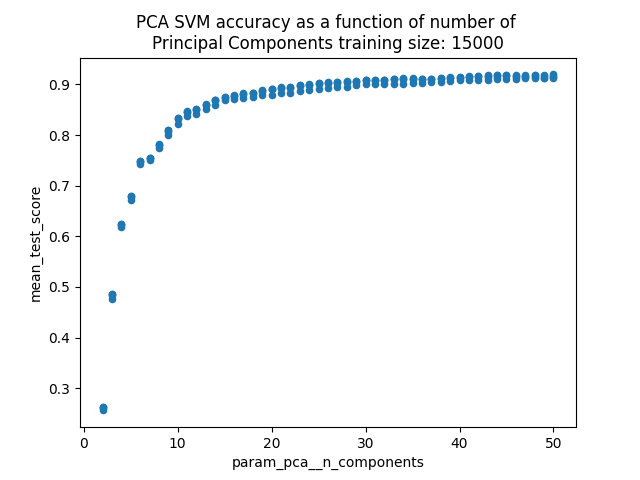
\includegraphics[width=0.8\textwidth]{figures/experiment_two/pca_svm_15000.png}
    \caption{Accuracy of the SVM model with \gls{pca} as dimensionality reduction method, with the number of components used.}
    \label{fig:experiment_2_pca_svm}
\end{figure}

For \gls{pca}, the highest accuracy value is 91.99\% with 50 components and the value 0.01 for the C hyperparameter in \gls{svm}. The thresholds for \gls{pca} are: 91.99 - 1\% = 91.07, 91.99 - 5\% = 87.39, and 91.99 - 10\% = 82.79. The results of the experiment for \gls{pca} will be compared to these thresholds.

By sorting the data by \texttt{mean\_test\_score} and going through the values, given the best-case scenario with the best hyperparameters found. The first value that drops below the threshold of 91.07\% is with an accuracy of 90.57\% at 29 components, which means that the model's accuracy only increases by 1\% with the last 21 components, which is close to half the total amount of components.
The next threshold of 87.39\% accuracy is found at 86.86\% with 14 components. By removing an additional seven components, the accuracy dropped from a 1\% loss to a 5\% loss.
The final threshold of 82.79\% accuracy is found at 80.70\% with nine components. By removing only five components, the accuracy dropped from a 5\% loss to a 10\% loss.

\subsubsection{Linear discriminant analysis}\label{subsubsec:experiment_2_lda}
The scatter plot representing \gls{lda} method can be seen in \autoref{fig:experiment_2_lda_svm}. \gls{lda} reduces the dimension to the number of classes $-1$, which is why the total number of components used is nine since \gls{mnist} has ten different numbers. The general trend is still valid for discussion in the second experiment.


\begin{figure}[htb!]
    \centering
    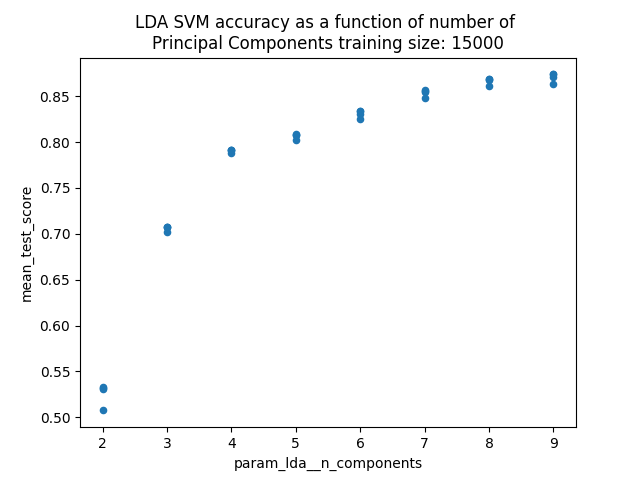
\includegraphics[width=0.8\textwidth]{figures/experiment_two/lda_svm_15000.png}
    \caption{Accuracy of the SVM model with \gls{lda} as dimensionality reduction method, with the number of components used.}
    \label{fig:experiment_2_lda_svm}
\end{figure}

For \gls{lda}, the highest accuracy score is at 87.38\% with nine components and the value 0.1 for the C hyperparameter in \gls{svm}. The thresholds for \gls{lda} are: 87.38 - 1\% = 86.50, 87.38 - 5\% = 83.01, and 87.38 - 10\% = 78.64. The experiment's results for \gls{lda} will be compared to these thresholds.

Repeating the method of looking through the data gathered, the first value that drops below the first threshold  of 86.50\%, with the 0.1 hyperparameter, is at 85.61\% with seven components.

The next threshold of 83.01\% accuracy is found at 80.83\% with five components. By removing two components, the accuracy dropped from a 1\% loss to a 5\% loss, which is not many components when compared to \gls{pca}, but for \gls{lda} that only has nine total components, a large percentage of the components can be removed with only a 5\% accuracy loss.

The final threshold of 78.64\% accuracy is found at 70.75\% with only three components. They are showing a significant drop from the threshold since the first few components impact the accuracy score significantly, and the closest value to the threshold is ~8\% away.


\subsubsection{\gls{kpca}}\label{subsubsec:experiment_2_kpca}
\gls{kpca} is a nonlinear dimensionality reduction method, and the scatter plot representing this method can be seen in \autoref{fig:experiment_2_kpca_svm}.

\begin{figure}[htb!]
    \centering
    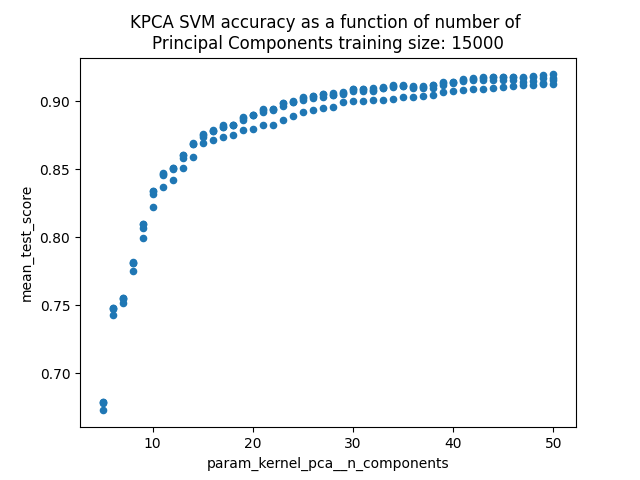
\includegraphics[width=0.8\textwidth]{figures/experiment_two/kpca_svm_15000.png}
    \caption{Accuracy of the SVM model with \gls{kpca} as dimensionality reduction method, with the number of components used.}
    \label{fig:experiment_2_kpca_svm}
\end{figure}

\autoref{fig:experiment_2_kpca_svm} is very similar to the other methods, and almost identical with \autoref{fig:experiment_2_pca_svm}, the only difference is that \gls{kpca} uses at minimum 5 components, where \gls{pca} uses at the lowest 2 components.

\gls{kpca} has a top accuracy score of 91.99\% with the value 0.01 for the C hyperparameter in \gls{svm}, meaning that the thresholds for \gls{kpca} are: 91.99 - 1\% = 91.07, 91.9 - 5\% = 87.39, and 91.9 - 10\% = 82.79. The experiment's results for \gls{kpca} will be compared to these thresholds.

Similar to linear methods, the data is sorted by its accuracy score to find the first value where the accuracy drops below a threshold, that uses the same hyperparameter. The first threshold of 91.07\% accuracy is found at 91.04\% with 34 components. The next threshold of 87.39\% accuracy is found at 86.86\% with 14 components. The final threshold of 82.79\% accuracy is found at 80.70\% with nine components.


\subsubsection{\gls{isomap}}\label{subsubsec:experiment_2_isomap}
\gls{isomap} is the final method of the second experiment, which is nonlinear, and the scatter plot representing this method can be seen in \autoref{fig:experiment_2_isomap_svm}.

\begin{figure}[htb!]
    \centering
    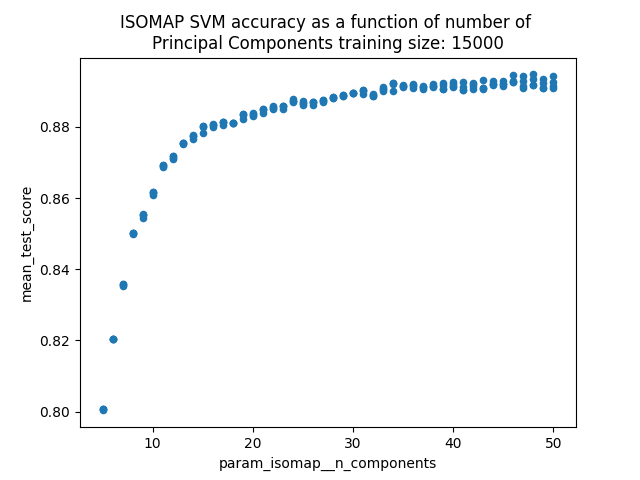
\includegraphics[width=0.8\textwidth]{figures/experiment_two/isomap_rerun_svm_15000.png}
    \caption{Accuracy of the SVM model with \gls{isomap} as dimensionality reduction method, with the number of components used.}
    \label{fig:experiment_2_isomap_svm}
\end{figure}

\autoref{fig:experiment_2_isomap_svm} is similar to the other methods as the accuracy drops drastically as the number of components decreases, but interestingly even the lowest accuracy for \gls{isomap} is still relatively high. The span from best to worst accuracy is much smaller than the other methods. The highest accuracy score for \gls{isomap} is 89.4\% with 48 components and the value 0.001 for the C hyperparameter in \gls{svm}, and the lowest accuracy score is 80\% with five components. The best and worst accuracy scores are closer together than the other methods, with only a ~9\% difference.

isomap has a top accuracy score of 89.47\%, with 48 components, and the value 0.001 for the C hyperparameter in \gls{svm}. meaning that the thresholds for \gls{isomap} are: 89.47 - 1\% = 88.57, 89.47 - 5\% = 84.99, and 89.47 - 10\% = 80.52.

The first threshold of 88.57\% accuracy is found at 88.49\% with 22 components, the next threshold of 84.99\% accuracy is found at 83.54\% with seven components, and the final threshold of 79.4\% accuracy is not found in the data, as the lowest accuracy score is 80.8\% with five components. To still be able to compare the results of \gls{isomap}  with the other methods, the lowest accuracy score will be used as the threshold, but it should be made clear that the actual threshold is not found in the data.


\subsection{Discussion of experiment 2}\label{subsec:experiment_2_discussion}
This section will discuss the results of the second experiment and compare the results of the different methods, first by discussing the results of the linear methods, then the nonlinear methods, and finally, comparing the results of all methods.

For each section, a table will display the different percentages of components remaining before the accuracy drops below a threshold. The table will also show the number of remaining components to show the difference between the methods.


\subsubsection{Linear methods}
By comparing the two linear methods used for the second experiment, it is essential to know that the number of components is very different between \gls{pca} \gls{lda}, which means that an exact comparison between the two methods is not always clear. Instead of using the number of components as a comparison, the percentage of remaining components will be used to try and make a fair comparison. A table showing the differences between the two methods can be seen in \autoref{tab:experiment_2_linear_methods_comparison}.

\begin{table}[htb!]
    \centering
    \begin{tabular}{cp{0.15\textwidth}p{0.15\textwidth}}
        \toprule
        \textbf{Thresholds} & \textbf{PCA \% 50} & \textbf{LDA \% 9} \\
        \midrule
        1\%                 & 58\% (29)          & 77.7\% (7)        \\
        5\%                 & 28\% (14)          & 55.5\% (5)        \\
        10\%                & 18\% (9)           & 33.3\% (3)        \\
        \bottomrule
    \end{tabular}
    \caption{Percentage of the components remaining after the threshold is reached, with the corresponding number of components in paratheses.}
    \label{tab:experiment_2_linear_methods_comparison}
\end{table}

\autoref{tab:experiment_2_linear_methods_comparison} shows, for each linear method, the amount of components left after each of the thresholds is reached. So for \gls{pca}, 58\% of the total number of components remain before reaching the first threshold of 1\%, whereas, for \gls{lda}, there is 77.7\%.

From \autoref{tab:experiment_2_linear_methods_comparison}, it can be seen that before reaching the first threshold of losing 1\% accuracy, \gls{pca} can cut off 42\% of its components, while \gls{lda} can can only cut off 22.3\%.

By comparing the two linear methods, it can be concluded that \gls{lda} is more prone to losing accuracy when removing components than \gls{pca}. The accuracy loss is likely because \gls{lda} has so few components to work with in the first place. It could be argued that the results are not entirely fair since \gls{pca} has so many more components, but scaling the values with percentage should show a general trend.


\subsubsection{nonlinear methods}
Unlike the linear methods, the nonlinear methods have a similar number of components, which should give a more fair comparison. A table showing when the respective thresholds were reached for each of the nonlinear methods can be seen in \autoref{tab:experiment_2_non_linear_methods_comparison}.

\begin{table}[htb!]
    \centering
    \begin{tabular}{cp{0.20\textwidth}p{0.20\textwidth}}
        \toprule
        \textbf{Thresholds} & \textbf{KPCA \% 50} & \textbf{ISOMAP \% 50} \\
        \midrule
        1\%                 & 68\% (34)           & 44\% (22)             \\
        5\%                 & 28\% (14)           & 14\% (7)              \\
        10\%                & 18\% (9)            & 1\% (5)*              \\
        \bottomrule
    \end{tabular}
    \caption{Percentage of the components remaining after the threshold is reached, with the corresponding number of components in paratheses.}
    \label{tab:experiment_2_non_linear_methods_comparison}
\end{table}

Figure 1 shows that \gls{kpca} and \gls{isomap} can afford to cut off a significant amount of components before reaching the first threshold of 1\%. \gls{kpca} can cut off 32\% of its components, while \gls{isomap} can cut off 56\% of its components. Another interesting note is that \gls{isomap} never reaches the 10\% accuracy loss threshold, and the closest accuracy score is used instead. Although it is not entirely accurate, the percentage from the actual threshold is <1\%, so for the sake of the comparison, it will be assumed that the threshold was reached.

Generally, it can be concluded that both \gls{kpca} and \gls{isomap} can afford to cut off a significant amount of components before losing accuracy. It is interesting to note that \gls{isomap} can cut off more components than \gls{kpca} before losing accuracy. However, \gls{kpca} reaches a higher accuracy score than \gls{isomap} but also reaches a lower accuracy score than \gls{isomap}, which means that \gls{isomap} could be considered more consistent than kpca, as the span of accuracy score for \gls{isomap} is smaller.


\subsubsection{Comparison of methods}
Now that the linear and nonlinear methods have been compared, it is time to compare the methods to each other. The results can be seen in \autoref{tab:experiment_2_methods_comparison}.


\begin{table}[htb!]
    \centering
    \begin{tabular}{cp{0.15\textwidth}p{0.15\textwidth}p{0.15\textwidth}p{0.20\textwidth}}
        \toprule
        \textbf{Thresholds} & \textbf{PCA \% 50} & \textbf{LDA \% 9} & \textbf{KPCA \% 50} & \textbf{ISOMAP \% 50} \\ \midrule
        1\%                 & 58\% (29)          & 77.7\% (7)        & 68\% (34)           & 44\% (22)             \\
        5\%                 & 28\% (14)          & 55.5\% (5)        & 28\% (14)           & 14\% (7)              \\
        10\%                & 18\% (9)           & 33.3\% (3)        & 18\% (9)            & 1\% (5)*              \\
        \bottomrule
    \end{tabular}
    \caption{Percentage of the components remaining after the threshold is reached, with the corresponding number of components in paratheses.}
    \label{tab:experiment_2_methods_comparison}
\end{table}

The first noticeable thing is that \gls{pca} and \gls{kpca} are similar in the number of components they can cut off before losing accuracy enough to reach the thresholds. The highest accuracy score is the same between the two methods, but the lowest accuracy score is lower for PCA, this lower accuracy score is likely due to the range of components \gls{pca} has. The lower the percentage in \autoref{tab:experiment_2_methods_comparison}, the more components can be cut off without losing accuracy. So from this, it can be concluded that \gls{lda} is the method that has the most drastic accuracy loss when cutting off components. This is likely because \gls{lda} has so few components to work in the first place, and therefore it is more sensitive to the removal of components. \gls{isomap} is the method that has the most negligible accuracy loss when cutting off components. Additionally, \gls{isomap}'s worst accuracy score is better than any other method, but its best accuracy score is also the lowest.

From the second experiment, it can be concluded that \gls{isomap} is the method that can cut off most components before losing accuracy. However, each method has its strengths and weaknesses, and it is essential to consider the context of the problem when choosing a method.


% intro
% presentation af de experimenter vi har valgt og hvorfor vi har valgt dem?
% experiment 1 exemple
%     detaljeret gennemgang af regler og evaluering
%     fremvisning af resultater
%     opsumering af resultater
%     diskussion af resultater og hvad der ellers var spændende evaluering af hvorfor det blev sådan.

%logarithmic regression
%Bar chart